% This example An LaTeX document showing how to use the l3proj class to
% write your report. Use pdflatex and bibtex to process the file, creating 
% a PDF file as output (there is no need to use dvips when using pdflatex).

% Modified 

\documentclass{l3proj}

\begin{document}

\title{Cesium Mapping Project - Team CS16}

\author{Harry Goodwin - 2557827G \\
        Adam Fairlie - 2461352f\\
        Philip Coffey - 2462160c\\
        Faraj Ahamed Monnapillai Ahamed Nagoor - 2465104M}

\date{21 March 2022}

\maketitle

\begin{abstract}
This paper will analyse and document the development of a large scale mapping web app for the multinational company Thales.  It will do this through discussing software practices in an agile environment, reflecting on problems and how they were overcome.  The bulk of the case study will be regarding our reflections in this development life cycle, with conducting customer meetings, integrating the software together, finding information on how to implement technologies and implementing new software practices.  With these reflections, an emphasis on the key themes, lack of experience with software practices, building this type of web app and lessons learned.  The case study will then conclude with a summation of what has been discussed in the case study.


\end{abstract}

%% Comment out this line if you do not wish to give consent for your
%% work to be distributed in electronic format.
\educationalconsent

\newpage

%==============================================================================
\section{Introduction}
\setlength{\parindent}{20pt}

This paper presents a case study of a university development project spanning 7 months.  The project is designed to simulate a realistic environment in which a development team will function in the real world.  It attempts to achieve this goal through certain factors, mainly the use of real customers and pushing the use of modern software development processes by marking their use.  Another factor to improve the realism of the project was to have a huge range of projects that could be assigned, this would minimise any collusion that could take place ensuring that teams found their own way. \par
The app developed was an offline mapping application like google earth, this tool would then be used to show where troops are situated on the earth, or plan troop movements on the earth.  Therefore, the key functional requirements laid out were that an offline mapping tool must be produced which could simulate the movement of icons, and different layers could be drawn and/ or applied. \par

\begin{figure}[h]
\begin{center}
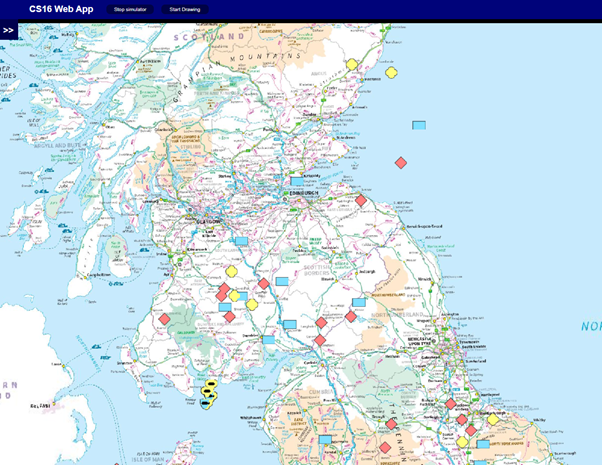
\includegraphics[width=\textwidth]{images/Picture1.png}
\end{center}
\caption{A screenshot of our final app}
\label{fig:app}
\end{figure}

This case study will document those key experiences gained from the team project.  Experiences in many different areas of software development, teamwork, agile development, testing, design, interactions with a real customer, set-backs, conflict resolution, and many more.  Generally, it will relate problems that arose, how they were dealt with, what was learned and how these lessons helped to improve the overall state of the project.\par

To illustrate the educational experience gained through developing this application, the document will be structured as follows.  Firstly there will be a section documenting an in-depth background of the case study as well as motivations for creating such an app.  Secondly the bulk of the case study will be made up of reflections in 4 different areas.  The first reflection will discuss how the team improved its interactions with the customer.  Secondly integration of each software element of the overall project.  Thirdly research into the many new languages, frameworks and technologies and finally usage of modern software practices.  The case study then finishes with a conclusion summing up what has been learned.

Through this structure, detail and referencing a clear picture will be generated of the steps followed in order to create this app and the lessons learned along the way. 

%==============================================================================
\section{Case Study Background}

The customer was a project manager “Matt Tucknott”,  working for the French multinational “Thales”, which specialises in electrical systems for aerospace, defence, transportation, and security markets.  Matt’s area of expertise within Thales is creating mapping systems, like Google Earth.  These mapping systems feature terrain, in-depth layers of cities, roads and tracks and simulators that can move military standard symbols around the maps. He wanted to show to Thales that the software that they spend a lot of money to produce, could be produced using free open-source software.\par
Subsequently the initial brief consisted of the functional requirements: the app must work offline, contain a simulator, be able to toggle layers, be able to draw shapes, and feature world terrain.  Matt's most important requirement was that the app had to work offline; this was because it had to work in the field where perhaps there won’t be reliable access to the internet.  The simulator was important to show how the offline server could handle the rapid movement of over 1000 APP6 icons.  APP6 is NATO's joint military symbology.  Layers were required to toggle some features, such as highlighting roads and tracks.  Drawing shapes simply would allow any user to highlight areas on the maps.  Terrain was important as without it obviously the earth is just flat, no kind of movement could ever be simulated or envisioned on the map without it.  In short Matt wanted an offline web app that could rival Thales’s product with open-source technologies. \par
Furthermore, this product was going to prove to be a challenge as there was no experience in the group with building software such as this, working in a team on a project of this scale or with the languages/ technologies that were going to be involved, notably JavaScript and Cesium.  The core open-source technology that formed the backbone of the app had many example scripts that detailed how to create drawing, layering and simulation functionalities.  As for generating APP6 symbols, these are very widely used and didn't pose much of a problem.  Ensuring the app worked offline with offline maps and offline terrain posed a big challenge, mostly because of the lack of/ conflicting documentation online of how to achieve this goal.  In summary every one of Matt's functional requirements was achieved, some being more of a challenge than others.\par
Putting it all together, the goal was to prove to Matt and Thales that their software could be recreated using open-source software found online.  Success would also show that it would need little to no training to build an application with these technologies as was demonstrated.  Essentially if the project was a huge success, it could be used to revolutionize the way in which Thales creates its software, saving the company a lot of money.  Although, because Thales is building military grade software, software found in open-source libraries might not be the most suitable as it could contain malicious code or careless bugs.  Thales would have to spend more time checking the credibility of code before they decided to go with its implementation and use or vet the developers whereas because we are students the concern is more so to get the app working.





%==============================================================================
\label{sec:Customer}
\section{Conducting customer meetings}
Over the course of this project my team and I participated in 5 official customer days, and 3 smaller unstructured meetings, which just involved us asking our customer a few clarifying questions. Through these 5 customers days we gradually altered our approach to these meetings, using a combination of the feedback our marker gave us, along with our own reflections about what worked well and where we could make improvements. \par
Our first meeting with our customer was on the 13th of October. This meeting did not have any marks attributed. The first thing we did was discuss what our goal for the meeting was. All 4 of us were struggling to get a clear mental picture of the app that we were being asked to develop. So, we went through the presentation given to us and created a list of questions, that we believed would help clarify some of our points of confusion.\par
The meeting overall was very successful. We asked all our questions within the time frame and the answers we received were clear and concise. Our stated goal of understanding the project was achieved as we spoke after the meeting and me and my team had a much better grasp on our assignment. As we ended the meeting, we briefly discussed what our goals are for the next meeting, which was essentially just us agreeing to look up some of the technologies recommended in the provided specification. This was quite a simple meeting when compared to what our later meetings would become. Although, this meeting was an important example to us about how useful communication with our customer can be, as our confidence in our ability to complete this project was significantly improved in just 20 minutes of talking.\par
In the days following our first customer meeting, my team and I spoke about some points of improvement we could make for our first marked assignment on the 10th of November. We felt like the meeting was a bit messy as we would sometimes talk over each other. To solve this, we assigned a designated chair to keep the meeting under control. It was also our opinion that the sprint goals were not defined clearly enough. To improve upon this, we decided to have a section at the end of the meeting dedicated to what we were planning on doing for the next sprint.\par
Being our second meeting, we had the added responsibility of communicating the progress we had made. Which was of course, not something we needed to worry about in our first meeting. We decided it was best to set a dedicated demonstrator who would take the customer through a PowerPoint, where we had listed all the key information we had found out throughout our sprint. We also gave our opinions on which technologies would be best for developing the project. As planned, after the demonstration, we listed our goals for the coming sprint and then asked our customer if he had any questions, which he did not. From this meeting we learned that having a dedicated chair makes the conversations flow much better, so we continued assigning a chair for the rest of our meetings. We also learned that having a visual representation of the information that we were communicating, makes it easier for the customer to understand. We determined this because, the most effective section of the meeting was the demonstration, which utilised a PowerPoint.\par
Following the meeting our marker gave us some advice by recommending the chair uses a PowerPoint for their sections. The meeting also felt very one way, as the customer was not very involved in the discussion. To improve upon this, we put more thought into how we presented our opinions on where to take the project, with the goal of leaving more opportunities for our customer to give his input on our decisions. Overall we were pretty happy with this meeting as we got high praise on the demonstration section, and we came away with several ideas of how to improve for next time.\par
Our third customer meeting took place on the 1st of December. We took the time to make a PowerPoint to display the recap at the beginning, along with the sprint plan at the end of the meeting. The information we wanted to communicate to our customer was the somewhat functional app that we had developed during the sprint. To show this, we designated a demonstrator to screen share as they loaded and used the app that we had made. We decided to keep the same chair and demonstrator throughout all of the meetings, as swapping roles could make it difficult for the customer to recall prior meetings if our voices didn't match.\par
As this meeting was taking place just before the Christmas holiday, we decided to be more ambitious in this sprint, as we would not have any other assignments to worry about. Instead of just listing our plans as before, we wanted to give our customer more input so we created a list of all possible tasks we could begin working on and we then asked our customer to group these tasks into high, medium or low priorities. This was successful in the sense it got our customer much more involved than our previous method. Although as pointed out by our examiner, we still did not have the clearest outline of the tasks we would attempt to complete, just a general plan to focus on the high priority issues.\par
Although we definitely felt like we were getting better at this, we still had some things we wanted to change for our 4th customer day. First our examiner pointed out that our recap was very brief, and we agreed. To solve this, we just needed to make sure to go into more depth in the recap, as we had time to spare this wasn’t a problem. We also decided it could be a good idea if we changed the way that we did our demonstrations. To run our app the user just has to download the files then run an executable and the app would start. We wanted to exploit this simplicity and get our customer to run the app at the beginning of the meeting, then when it came time for the demonstration, we would ask him to share his screen, and our demonstrator would talk him though the features. From this, we leaned that having a interactive demonstration brings multiple benefits to a meeting. The customer came away with a better understanding of our features than he had prior, and he ended up giving us a couple direction on how he would like us to adjust the app, which he had not done in our previous demonstrations.\par
Leaving our 4th meeting, we once again made a plan for the upcoming sprint. This time we made sure to explicitly say which features we would work on, along with a couple stretch goals. In my opinion, this meeting represented the biggest improvements we made throughout the course, as it felt like the points of improvement were becoming much more minor. The only pressing issue that was pointed out to us was, some other groups dedicated a section of the recap to explicitly stating their progress against the goals. Up until this point we had been keeping our recap of goals and progress demonstration separate, but we all agreed it would be useful for our customer to see these 2 pieces of information compared.\par
Going into our 5th and final customer day (not including the final demonstration), we kept much the same from our previous meeting, with the added detail of comparing our progress to our goals in our recap. This meeting was also slightly different in the sense that it was our final official meeting, so we need to make sure our sprint plan was as accurate to our customer requests as possible, as we may not have the opportunity to fix mistakes made in this final sprint. To do this we dedicated more time to the sprint plan than we did before, and we had one of our team members write up the list of goals during the meeting, so we could show the customer them, to give him as clear a picture of our plan as possible.\par
Being the final customer day, this brings us to the end of our reflections on our customer meetings. To conclude, we went from not really thinking beyond setting a broad goal and just trying to achieve that within our time. By the end we were thinking about our meetings as a set of goals that include providing our customer context for the meeting so they can understand what we’re talking about, then giving as clear and concise of a progress report as possible. Only once the customer has been completely caught up, we would then take time to agree on the best path forward by making it as easy as possible for our customer to express their opinion openly without any pressure. In my opinion we have made good progress in the way we viewed these meetings, and we believe that a lot of the success we had in this assignment specifically came from our attempts to make the most of our customer meetings.\par


\label{sec:Software}
\section{Integrating the software together}
After the initial meeting with the customer, where elements of the brief were clarified and a detailed overview of the project details were established, the next step for our team was to research the free and open-source technologies available for the different components of our project and how they can be linked together to produce the final app. We used our first sprint to decide on the software to use for the back-end map server and the web front end to show 2D maps and 3D globes in an offline web app environment. It became clear at the early stages of this research that with the constraints given by the customer, the technologies used in our app would have to operate using multiple different languages and set-ups, and we would have to find a way to carefully integrate them together. When investigating map servers available, we found that the most powerful and reliable programs available to us, GeoServer and MapServer, are written in Java and C/C++ respectively\cite{GeoServer}\cite{MapServer}. We also considered PyGeoAPI, written in Python, however we quickly decided that the lack of documentation and industry use made it the inferior choice for our purposes. All of the front-end web-based options we looked at \cite{CesiumJS}\cite{WorldwindWeb}\cite{GEEnterprise}\cite{Maptalks} were libraries for JavaScript, which is the natural choice for a web-based front end.\cite{JSUses} The final choices we made were GeoServer and CesiumJS.

Integrating these technologies together was something our team found difficult, and after some failed attempts we found a way to use Apache Tomcat, a Java-based web server which allowed different apps to run on a local server\cite{Tomcat}. This setup allowed us to download the GeoServer web archive (WAR) and run it as an app on the server, and have a separate app hosting an HTML webpage, which we could program with JavaScript to set up a 3D globe with the Cesium library. Initially this was the perfect solution: we could have both technologies running on the same environment and access them both with different named URL’s, start and stop them both simultaneously, and easily bring GeoServer shapefiles into Cesium by querying the locally hosted server. This process taught us many valuable lessons about how to find useful tutorials and forum posts to troubleshoot and how to quickly gain an understanding of unfamiliar technologies and frameworks.

The major integration issues came quickly after the setup, when we began developing the project features and considering how to test our code. We found that almost all JavaScript testing is done through Node.js, and after some research we decided to use the most popular testing library, Jest. The compatibility issues were immediately obvious when we tried to write our first tests. Jest was made to test modular, self-contained code. The code we had written for the app so far relied on all our files being loaded in the HTML file and using global variables and methods to give each JavaScript file the information needed to implement its functionality. We have learned for future projects the importance of taking the extra time initially to ensure our code is scalable, testable and easy to read, which will save time and effort overall.

Extensive refactoring was done to split our functionality into mostly self-contained modules which shared functionality through importing functions and classes, and this allowed for some features to be tested, but the limitations of Jest in simulating the web-based environment of our project became obvious and ultimately limited what functionality could be properly tested.

The largest problem we encountered while trying to run tests on our JavaScript code however, was the integration of Node.js testing libraries with code written for a web browser. When first trying to run written tests on our code, we found that the test files had trouble importing the code we’d written for modules of our app and gave us an error that the imports were undefined. Upon some research into this problem, we discovered that this is because web browsers and Node.js apps use a different JavaScript standard, with different syntax for importing and exporting classes and methods. JavaScript modules are a relatively new feature to web browsers, and the imports and exports used follow the ES6 code standard, with keywords “import” and “export”. Node.js uses the older CommonJS standard, which uses “require” to import modules. Web browsers have no way to handle CommonJS imports and throw an error, and similarly the Node.js test suite cannot easily import an ES6 module\cite{CommonVsES6}. 

Testing libraries, including Jest, do offer some support for testing ES6 modules \cite{JestES6}, but in our web app the conversion is incomplete, and at some point when importing the Cesium libraries it again begins not to recognise the ES6 import style. This syntax clash was the cause of major issues for a month-long period, with many different solutions tested which at best provided a partial solution which allowed for us to test a restricted amount of our app. Eventually, we found a solution through a Node.js plugin called Babel, which converts all files to CommonJS before running the tests\cite{Babel}. This allows for us to test any part of the code, but means that running the test suite takes several minutes to complete the conversion of many different files from libraries used in our project, meaning our pipeline was very slow.

Many of these integration difficulties felt unavoidable due to our lack of experience, as we knew early into the project, but others – particularly with testing – we believe were a result of a lack of comprehensive planning. During our research phase, where we planned the technologies and how to bring them together, testing was left as an afterthought. We only put serious thought into testing after substantial work had been done implementing many of the core features of our app, and this led to the need for major refactoring halfway into the project when the code base was beginning to grow very large, and the inability for us to properly test certain aspects of our project, particularly the 3D-based elements. By the time we gained an understanding of the issues related to testing our app, many of the potential solutions we came across involved a major change to the technology stack of our app, something which was infeasible at that stage in the project. 

If we had discovered in our research and planning that testing was mostly done through Node.js, we could have adopted a tech stack which incorporates it more heavily from the start. Instead of using plain HTML with the Tomcat web server, we could have gone with an approach using react, a JavaScript library which works with Node.js and can be used to create webpages and host on a server\cite{React}. This was initially dismissed due to the extra difficulty, which we thought was unnecessary during planning, however in hindsight this approach would have had many advantages. It would have allowed for far more seamless integration of components, as Cesium and milsymbol (the library for generating APP-6 symbols) could have been directly imported through Node.js, and testing would have been far quicker and easier as all files would be written in the CommonJS standard, with no need for conversion. This would have been a more logical set-up for the project, using Node.js to bring all JavaScript elements together rather than as a framework added on top of our initial project to write some tests.

In future projects, we would extend our research to considerations such as testing and code layout, instead of stopping prematurely at how to make the first working prototype. I believe our team was anxious to provide something demonstrable using technologies we had no experience in and focused too heavily on setting up the app and adding features as quickly as possible to impress the customer. This was important to us, as it helped us maintain the customers trust in our abilities to deliver, but the short-sightedness of our original research made it harder to deliver in future meetings. We feel these invisible considerations are just as important to a successful software project, to ensure our code is reliable and robust. The importance of trusting the ability of our software to do what it advertises accurately is incredibly important, especially in a project such as this, in which failures may have serious real-world implications. If these problems were identified before they could manifest in the project, we could have discovered a more sensible set-up and streamlined the development process, delivering more to the customer overall.

\label{sec:Research}
\section{Finding information on how to implement technologies}
Throughout the design, development and testing of the app, many issues arose.  These issues came to fruition because of a lack of prior experience with the technologies being implemented, with software development processes, with testing and with design.  This section of the case study will examine these issues and how they came to be resolved through research and issues with research methods utilized. \par
The first notable issue that the team came across was attempting to find material that documented the process of building an offline app such as the one requested.  There was a lot of documentation online about how to manufacture such an app, but far less on how to develop it offline.  The team spent several weeks branching off in different directions, trying to find information on how to implement.  The first relevant guide that emerged was \cite{DaleBingham}.  This guide at first appeared to include everything required: map server, offline use, and basic setup.  It documented the steps in which Bingham took to create an offline mapping app, the technologies used and how they were implemented.  It didn't take long until setup issues began to arise whilst following the guide, notably different versions of the technologies being used had to be installed on each instance, making implementation and collaboration completely unfeasible.  After struggling with this guide for several weeks, 2 YouTube videos emerged \cite{OpenGeoLab} \cite{WebGISDev}.  This video showed the steps in creating a compartmented version of the app, albeit online, but it was progress.  In reflection, the method of splitting the team up to research like this showed inexperience in large team working projects.  Communication wasn't very strong this early on meaning as people branched, others in the group were less aware of the direction the project was taking.  A method to overcome this distancing was learned later in the course: to do weekly stand-up meetings that helped to keep everyone on the same page with progress and thought channels. \par
Subsequently once the bare bones of the app had been created, it was a matter of implementing the requirements on top of this setup, drawing shapes, layering and a simulator.  These tasks didn’t pose much of a challenge.  This is firstly because the quality of the information found on these topics online was abundant and of good quality.  With shape drawing and layering, demos and example code of how to implement appeared on Cesium Sandcastle\cite{CesiumSandcastle}, which is an online version of the Cesium app that can be changed programmatically, and the results witnessed live.  Cesium sandcastle had many different code bases for different features, giving the opportunity to plainly see how the app functioned which assisted the implementation.  Here progress was good and speedy, because there appeared to be a singular, best way to conduct the implementation of these features as lots of people have done it before.\par
Eventually the problem of transitioning the app to offline emerged, this meant downloading maps to store locally and then serving these to the app.  Until now the app had been working in an online setting, taking all its map data from the Cesium websites map dumps.  Researching how to get offline maps to work turned into a massive challenge, spanning several months.  At first the thought was that simply that maps could be taken from a source and then inserted into the file tree of the app and visualised.  This did not work.  Research here began with trawling forums on the cesium website, this appeared to be a topic of some discussion among the Cesium community, with many solutions appearing in these forums\cite{OfflineMaps}.  This seemed very promising, as the thought process was that if there are many solutions, only one had to work.  However, either the answers where incomplete, wrong or outdated because none of the solutions found on the cesium blogs would work.  This became very frustrating as there was no experience within the group implementing something like this, and hence no credibility to fact check these blog posts and guides that where found.  This simply left the option to try everything suggested, which again was very frustrating as when implementations didn’t work as advertised, there was no indication if it was a mistake in the instructions, a mistake following the instructions or simply just incorrect/ outdated instructions.  A GitHub was found that had a guide on how to implement a low-resolution offline earth\cite{OfflineGuide}.  This was progress, but unacceptable for the final implementation.  After months of deliberations, we turned to Matt for advice as this is Matt’s areas of expertise. Not utilising his knowledge sooner was admittedly a mistake, but again this is an inexperienced team.  Matt assisted with what type of maps to use, and how to get them integrated into the app.  In addition the team could of put more of an emphasis on practices such as planning poker, this would of helped to gauge the difficulty in researching features such as this.  \par
After that there was the issue of adding terrain to the maps, which posed similar problems to the offline maps as there is an abundance of conflicting information online.  This meant that the same frustrating issues occurred of not knowing what was being attempted was the correct path.  The difference here was that the terrain was implemented after the maps and a valuable lesson had been learned in implementing the maps: the lesson to use any resources at our disposal, particularly Matt’s knowledge.  Matt directed the team towards 2 GitHub repositories, one for creating terrain from map data\cite{TerrainBuilder} and one for a server that would serve this terrain\cite{TerrainServer}.  The documentation for creating the terrain was relatively straight forward although for the server it was not.  Terrain had been successfully created with no way to visualise it.  Luckily, finding a guide that documented the creation of terrain and implementation of the terrain server was found in the comments of the GitHub repository, which helped immensely\cite{VisualTerrain}.  Whilst problems with research still showed here from the lack of experience, the lesson learned in the previous step illustrates a faster resolution to this problem. \par 
Lastly there were significant problems with setting up tests and the pipeline.  Again, like much of the project the team collectively had very little experience when it came to these aspects.  Luckily the university held a tutorial in setting up the pipeline and on effective testing, effectively solving any problems in these areas. \par
To conclude this section, research into unknown software development methods can be very frustrating, especially when possible solutions are documented poorly.  But this strain could have been alleviated if the customers knowledge had been utilized as a valuable asset in the development of the app.  More of an emphasis being put on utilizing software practices we had learned such as burn down charting and planning poker could of also helped to alleviate strain here as there could of been a faster resolution to these key problems if more members had been searching for solutions and collaborating.



\label{sec:Practices}
\section{Implementing new software practices}
In this section, we’ll speak more about the implementation of software practices we learned in the duration of this project, more than our implementation of the app itself.

\subsection{AGILE}
Throughout the project, we used different software practices to make each of our lives easier. Starting off, by using AGILE which allowed us to make sure that each one of us was up to date with our work for this project. We had structured weekly meetings with a time for a retrospective at the end of each meeting, where we discussed the current project objectives and priorities, and discussed; What we need to do less of, what needed to keep doing, what we need to do more of, and what we need to start doing. From research, we found that some of the risks with Agile practices are lack of customer engagement and poor team coordination, we made sure to tackle this problem by having the customer involved as much as possible. We had the customer join us in some of these meetings to gauge how we work and offer help and eliminate any problems or queries we might have had. Having the customer work so closely with us, made the work environment between us and the customer very calm and made the handover process very simple, as he had been pulling from the GitLab throughout the project timeline to test on their machine. 

We never got around to doing in-person scrum stand-up meetings, due to fact that none of us lived close to each other. The time taken for all to travel to one place would outweigh the negatives of having a short online meeting. Therefore, we decided to have a stand-up meeting online, which we only did a handful of times, as we found that it did not really for our team environment, instead, we just had informal meetings discussing how we are all getting along with our section of the project. Although, we did manage to have one in-person meeting during the second week of the project, as then some of us were closer together and had time to meet, which was helpful when it came to asking the question, but, we found that it wasn’t as productive as we thought it may be, therefore we stuck with online meetings from that point onwards.

At the start of the project, we set lose roles to each member of the team, but as we progressed, we found that the roles faded away and no one was particularly set to one role, as we all collaborated with each other, and everyone did a bit of all the roles listed in the scrum roles list. Although the role of product owner/primary contact was one member for the duration of the project, this was so that the customer always knew who to contact with confusion. This method seemed to work well for our team, so we decided to stick with this method of working.

\subsection{Issue boards}
We made use of issue boards for this, which are built into GitLab. We used the issue boards to keep track of the development process of the project by putting individual tasks into the following and moving them accordingly: backlog, under development, to be tested and closed (which indicates that we have completed that task). On top of this, we used a ranking system to show the importance of task completion, which we decided on ourselves but was always finalised by the customer, as we needed to match his needs for this project.

\subsection{Burndown chart}
Another feature we started using later in the project timeline to keep on top of work was a burndown chart [Figure \ref{fig:burndown}] created by our tutor, which shows the work left to do against the work we have left. This came in extremely useful, as we were able to see a visual rather than a text representation of our work in a timeline. It let us gauge if we needed to speed up work or were able to take a step back without affecting the completion time of the project, which removed a lot of stress when it came to time management. We would have preferred if we started using this earlier, but it was better late than never.

\begin{figure}[h]
\begin{center}
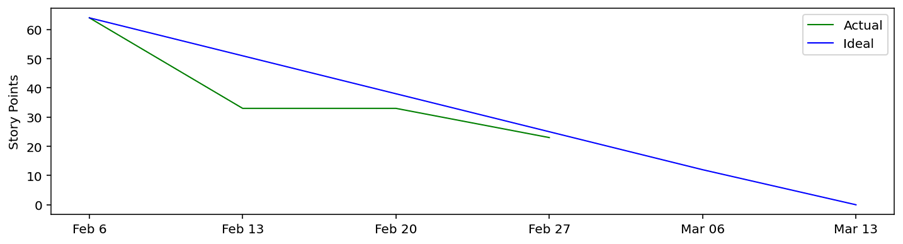
\includegraphics[width=\textwidth]{images/burndown chart.png}
\end{center}
\caption{Burn down chart}
\label{fig:burndown}
\end{figure}

\subsection{Continuous integration/continuous delivery (CI/CD)}
Continuous integration/continuous delivery was used in this project. This allowed us to build and test the code or file that is committed to GitLab automatically. There were a few benefits to implementing this feature, the obvious ones being timesaving during the testing phase and safely deploying the newly updated project into the old repository, and also less strain on the developer’s computers as the testing is being done online instead of the machine. The main drawback we had was during the set setup of the pipeline, as simply none of us had done this before and the amount of time used for research could have been spent somewhere more productive if the tutorial ran through the University was published sooner.

\subsection{Feature branching}
Feature branching came in extremely useful throughout the project, as it allowed us to separate the work evenly and allowed us to add to, modify and erase code or files without work overlapping or colliding with someone else’s work. Using features branching also meant that we had to take care of merge conflicts, but we found that this was only an issue at the start of the project, as later, everyone was working on different files, and there was not much overlapping.

\subsection{Testing}
When it came to testing our code, the structure in which the project had been created made it impossible to test. Meaning that there had to be extensive refactoring done before we could write any type of tests. When we were struggling to write tests, we did a few peer code reviews, not as much as we should have or hoped to, but still enough to where we all found it useful. Code reviews helped other members of the team understand what each other have written and how the software works, which made it helping each other a bit more pleasant. By the end of the project, we did manage to get tests written.

%==============================================================================

\section{Conclusions}

On the whole, this project proved to be incredibly challenging for every one of us, as this was the first time any of us knew of each other, and we have been put together to work on this long-term project, with no knowledge of how or what any of us are good at. We had to learn new languages and frameworks while maintaining a good software engineering practice in this team environment.

From the start of the project, we made sure that the workload was distributed equally among us, after taking each of our strengths and weaknesses into consideration. We did this by writing out the tasks that needed to be completed against the skill each of us attain or wanted to attain from this project, then we decided on which task each of us did. 

As mentioned before this is our team’s first long-term project and we believed at the start of the project collaborating with a large client such as Thales would be quite daunting, as the only skills or knowledge we have learnt so far is academically through a book and with no real-life practice. As we progressed on with the project, we were surprised to find out this was not the case, as Thales and Matt Tucknott were working and helping us each step of the each and were very understanding of any difficulties we were facing at any point of the project. This calming and friendly environment between us and the client made it so we were not only able to learn the technical side of a project like this, but also able to learn very valuable soft skills which all of us will be able to take with us in future projects.

At the very start of the project, most of us were fine with Gitlab as it was not complicated and was just recapping the building block which we have all learned previously. The difficulty started to build up when; branches, merge requests, GitLab runners, licensing, pipeline, etc, came into play, as this was the first time most of us used any of these types of features. This problem was put down promptly as we slowly watched and read up on the lectures that were being put out of the University. Although the lectures helped us when it came to configuring a GitLab CI/CD Pipeline, we did not manage to get this setup until extremely far into the project, again this was simply due to the lack of knowledge in this area, but after months of research and failure, this was also completed because of a tutorial hosted through the University.

To sum it up, we believe that we as a team have completed this project to the best of our ability with the knowledge and technology we had. We are satisfied with the results and the way we worked through the project, as the customer seems very content with the project and how we collaborated with him and had meetings with him outside the customer days throughout the whole project. Now at the end of the project, we can confidently say that we have a better understanding of how a project like this is worked on by industry professionals from start to finish, while also gaining knowledge of the technology we used from the wider industry. The few things we would have changed would be: making sure testing is set out properly from the get-go, using the burndown chart from the start of the project, and communicating better ourselves.

%==============================================================================
\bibliographystyle{plain}
\bibliography{dissertation}
\end{document}
